\documentclass[11pt]{article}\usepackage[]{graphicx}\usepackage[]{color}
%% maxwidth is the original width if it is less than linewidth
%% otherwise use linewidth (to make sure the graphics do not exceed the margin)
\makeatletter
\def\maxwidth{ %
  \ifdim\Gin@nat@width>\linewidth
    \linewidth
  \else
    \Gin@nat@width
  \fi
}
\makeatother

\definecolor{fgcolor}{rgb}{0, 0, 0}
\newcommand{\hlnum}[1]{\textcolor[rgb]{0,0,0}{#1}}%
\newcommand{\hlstr}[1]{\textcolor[rgb]{0,0,0}{#1}}%
\newcommand{\hlcom}[1]{\textcolor[rgb]{0.4,0.4,0.4}{\textit{#1}}}%
\newcommand{\hlopt}[1]{\textcolor[rgb]{0,0,0}{\textbf{#1}}}%
\newcommand{\hlstd}[1]{\textcolor[rgb]{0,0,0}{#1}}%
\newcommand{\hlkwa}[1]{\textcolor[rgb]{0,0,0}{\textbf{#1}}}%
\newcommand{\hlkwb}[1]{\textcolor[rgb]{0,0,0}{\textbf{#1}}}%
\newcommand{\hlkwc}[1]{\textcolor[rgb]{0,0,0}{\textbf{#1}}}%
\newcommand{\hlkwd}[1]{\textcolor[rgb]{0,0,0}{\textbf{#1}}}%
\let\hlipl\hlkwb

\usepackage{framed}
\makeatletter
\newenvironment{kframe}{%
 \def\at@end@of@kframe{}%
 \ifinner\ifhmode%
  \def\at@end@of@kframe{\end{minipage}}%
  \begin{minipage}{\columnwidth}%
 \fi\fi%
 \def\FrameCommand##1{\hskip\@totalleftmargin \hskip-\fboxsep
 \colorbox{shadecolor}{##1}\hskip-\fboxsep
     % There is no \\@totalrightmargin, so:
     \hskip-\linewidth \hskip-\@totalleftmargin \hskip\columnwidth}%
 \MakeFramed {\advance\hsize-\width
   \@totalleftmargin\z@ \linewidth\hsize
   \@setminipage}}%
 {\par\unskip\endMakeFramed%
 \at@end@of@kframe}
\makeatother

\definecolor{shadecolor}{rgb}{.97, .97, .97}
\definecolor{messagecolor}{rgb}{0, 0, 0}
\definecolor{warningcolor}{rgb}{1, 0, 1}
\definecolor{errorcolor}{rgb}{1, 0, 0}
\newenvironment{knitrout}{}{} % an empty environment to be redefined in TeX

\usepackage{alltt}
\usepackage{fullpage,graphicx,float,amsmath,enumitem,hyperref}
\setlist{parsep=5.5pt}
\setlength{\parindent}{0pt}

\usepackage{fancyhdr}
\pagestyle{fancy}
\lhead{Time Series Exam 1}
\rhead{Andrea Mack}
\setlength{\headheight}{24pt}
\setlength{\headsep}{2pt}

\title{Time Series Exam 1}
\author{Andrea Mack}
\date{November 09, 2016}
\IfFileExists{upquote.sty}{\usepackage{upquote}}{}
\begin{document}
\maketitle

\begin{knitrout}
\definecolor{shadecolor}{rgb}{0.969, 0.969, 0.969}\color{fgcolor}\begin{kframe}


{\ttfamily\noindent\color{warningcolor}{\#\# Warning: package 'stR' was built under R version 3.3.2}}\end{kframe}
\end{knitrout}



\begin{enumerate}
\item %1
{\it Complete the derivation of the autocorrelation function that was started for $Y_t$ in HW 7 number 7 (the derivation question that was not from CC). You can type up or handwrite any additional derivations required. Then plot the autocorrelation function (plot `type="h"` will be useful for this) using R. (7 pts)}


$\gamma_{o} = Cov(Y_{t},Y_{t}) = Var(Y_{t}) = 3$ from HW 7

$\gamma_{1} = Cov(Y_{t}, Y_{t-1}) = 2$ from HW 7

$\gamma_{2} = Cov(Y_{t}, Y_{t-2})$

= $Cov(0.5(x_{t-1} + x_{t}), 0.5(x_{t-3} + x_{t-2}))$

= $Cov(0.5x_{t-1}, 0.5x_{t-3}) + Cov(0.5x_{t-1}, 0.5x_{t-2}) + Cov(0.5x_{t}, 0.5x_{t-3}) + Cov(0.5x_{t}, 0.5x_{t-2})$  

Because pairs of $x_{t-i}$ with i $\geq$ 2 are uncorrelated, $\gamma_{2}$ reduces to

$0.5^2Cov(x_{t-1}, x_{t-2}) = 0.5^2 * 2 = \frac{1}{2}$

$\gamma_{3} = Cov(Y_{t}, Y_{t-3})$

= $Cov(0.5(x_{t-1} + x_{t}), 0.5(x_{t-4} + x_{t-3}))$

= $Cov(0.5x_{t-1}, 0.5x_{t-4}) + Cov(0.5x_{t-1}, 0.5x_{t-3}) + Cov(0.5x_{t}, 0.5x_{t-4}) + Cov(0.5x_{t}, 0.5x_{t-3})$  

= 0 because all time units are more than 1 unit apart.

Let k = the number of time units apart with $\rho_{k}$ the autocorrelation function.

\begin{equation*}
$\rho_{k}$ = 
\begin{cases}
$\gamma_o/\gamma_o = \frac{3}{3} = 1$ for k = 0\\

$\gamma_{1}/\gamma_{o} = \frac{2}{3}$ for $|k|$ = 1\\

$\gamma_{2}/\gamma_{o} = \frac{\frac{1}{2}}{3} = \frac{1}{6}$ for $|k|$ = 2\\

$\gamma_{3}/\gamma_{o} = \frac{0}{3}$ = for $|k|$ $\geq$ 3
\end{cases}
\end{equation*}




\item%2
\begin{enumerate}
\item%2a
{\it Derive the theoretical variance of a 3-point Moving Average built from an AR(1) process with normal white noise variance of $0.5^2$ and $\phi=0.4$ driving it. Again, this can be handwritten or typed. Your moving average is calculated as $Y_t=\frac{1}{3}(X_{t-1}+X_t+X_{t+1})$ where $X_t$ is the AR(1) process and you need to find $Var(Y_t)$. Your first step will be to sort out the variance and needed covariances for the AR(1) process based on results from when I introduced the AR(1) process. Show your work. (7 pts)}

$Var(Y_{t})$ = $\frac{1}{9}Var(X_{t-1}+X_t+X_{t+1})$ 

= $\frac{1}{9}[Var(X_{t-1}) + Var(X_{t}) + Var(X_{t+1}) + 2Cov(X_{t-1},X_{t}) + 2Cov(X_{t+1},X_{t}) + 2Cov(X_{t-1},X_{t+1})]$

= $\frac{1}{9}[3*\frac{1}{4} + 2*\frac{4}{10} + 2*\frac{4}{10} + 0]$

= $\frac{1}{9}[\frac{3}{4} + \frac{16}{10}]$

= $\frac{1}{9}[\frac{15}{20} + \frac{32}{20}]$

= $\frac{1}{9}[\frac{47}{20}]$

= 0.2611

\item%2b
{\it Use a simulation with 1,000 realizations of each process to check your answer for the variance of $Y_{t}$. The code below repeatedly simulates from this process and provides results of the estimated variance using time series with n=15 and n=300 observations. Summarize the mean and variability of the simulated results for each sample size to compare to the true result from part (a). (3 pts)}

The theoretical variance was 0.2611 and the simlation variance of the variances was 0.01 for a sample size of 15 and less than 0.01 for the sample size of 300. The discrepancy comes in because in #2b the variances found represent the variance of variances of sample size 15 and 300. To make #2a and #2b comparable, I can divide the result in #2a by 15 and 300 respectively, and I end up with more similar variances in the theoretical and simulation parts of #2. 

0.2611/15 = 0.0174

0.2611/300 = 0.00087

\begin{kframe}
\begin{alltt}
\hlstd{var15}\hlkwb{<-}\hlstd{var300}\hlkwb{<-}\hlkwd{matrix}\hlstd{(}\hlnum{NA}\hlstd{,}\hlkwc{nrow}\hlstd{=}\hlnum{1000}\hlstd{)}
\hlkwd{set.seed}\hlstd{(}\hlnum{1935}\hlstd{)}
\hlkwa{for} \hlstd{(k} \hlkwa{in} \hlnum{1}\hlopt{:}\hlnum{1000}\hlstd{)\{}
  \hlstd{var15[k]}\hlkwb{<-}\hlkwd{var}\hlstd{(}\hlkwd{na.omit}\hlstd{(stats}\hlopt{::}\hlkwd{filter}\hlstd{(}
    \hlkwd{arima.sim}\hlstd{(}\hlkwc{n}\hlstd{=}\hlnum{17}\hlstd{,}\hlkwd{list}\hlstd{(}\hlkwc{ar}\hlstd{=}\hlnum{0.4}\hlstd{),}\hlkwc{sd}\hlstd{=}\hlnum{0.5}\hlstd{),}
    \hlkwd{rep}\hlstd{(}\hlnum{1}\hlopt{/}\hlnum{3}\hlstd{,}\hlnum{3}\hlstd{),}\hlkwc{sides}\hlstd{=}\hlnum{2}\hlstd{)))}
  \hlstd{var300[k]}\hlkwb{<-}\hlkwd{var}\hlstd{(}\hlkwd{na.omit}\hlstd{(stats}\hlopt{::}\hlkwd{filter}\hlstd{(}
    \hlkwd{arima.sim}\hlstd{(}\hlkwc{n}\hlstd{=}\hlnum{302}\hlstd{,}\hlkwd{list}\hlstd{(}\hlkwc{ar}\hlstd{=}\hlnum{0.4}\hlstd{),}\hlkwc{sd}\hlstd{=}\hlnum{0.5}\hlstd{),}
    \hlkwd{rep}\hlstd{(}\hlnum{1}\hlopt{/}\hlnum{3}\hlstd{,}\hlnum{3}\hlstd{),}\hlkwc{sides}\hlstd{=}\hlnum{2}\hlstd{)))}
\hlstd{\}}
\hlcom{#why is n 302 and not 300, similarly with 17 and not 15?}


\hlstd{mean15} \hlkwb{<-} \hlkwd{mean}\hlstd{(var15)}
\hlstd{var15} \hlkwb{<-} \hlkwd{var}\hlstd{(var15)}

\hlstd{mean300} \hlkwb{<-} \hlkwd{mean}\hlstd{(var300)}
\hlstd{var300} \hlkwb{<-} \hlkwd{var}\hlstd{(var300)}

\hlstd{all} \hlkwb{<-} \hlkwd{data.frame}\hlstd{(}\hlkwd{matrix}\hlstd{(}\hlkwd{c}\hlstd{(mean15, var15, mean300, var300),}
                         \hlkwc{byrow} \hlstd{=} \hlnum{TRUE}\hlstd{,} \hlkwc{ncol} \hlstd{=} \hlnum{2}\hlstd{,} \hlkwc{nrow} \hlstd{=} \hlnum{2}\hlstd{))}
\hlkwd{colnames}\hlstd{(all)} \hlkwb{<-} \hlkwd{c}\hlstd{(}\hlstr{"Mean"}\hlstd{,} \hlstr{"Var"}\hlstd{)}
\hlkwd{rownames}\hlstd{(all)} \hlkwb{<-} \hlkwd{c}\hlstd{(}\hlstr{"15"}\hlstd{,} \hlstr{"300"}\hlstd{)}

\hlkwd{print}\hlstd{(xtable}\hlopt{::}\hlkwd{xtable}\hlstd{(all,} \hlkwc{align} \hlstd{=} \hlstr{"||r|r|r||"}\hlstd{,} \hlkwc{digits} \hlstd{=} \hlnum{4}\hlstd{))}
\end{alltt}
\end{kframe}% latex table generated in R 3.3.1 by xtable 1.8-2 package
% Wed Nov 09 15:17:56 2016
\begin{table}[H]
\centering
\begin{tabular}{||r|r|r||}
  \hline
 & Mean & Var \\ 
  \hline
15 & 0.1291 & 0.0069 \\ 
  300 & 0.1617 & 0.0005 \\ 
   \hline
\end{tabular}
\end{table}

\end{enumerate}

\item%3
{\it Ramsey and Schafer's Statistical Sleuth Section 15.2.2 (scanned pages available on D2L if you don't have a copy of the 3rd edition) presents a correction for autocorrelation for the standard error of the mean of a time series where you take the conventional SE estimate and multiply it by $\sqrt{\frac{1+r_1}{1-r_1}}$, so $SE_{corrected}=SE\sqrt{\frac{1+r_1}{1-r_1}}$ (in words in case compiling is rough, the multiplier to correct the SE is the square-root of ((1+$r_1$) divided by (1-$r_1$) )) where $r_1$ is the lag 1 sample autocorrelation estimate.}

\begin{enumerate}
\item {\it Find where the theoretical version of this result is discussed in CC and note the page and equation where they provided it. What assumptions about the error process are required for this to be the correct adjustment? Is this an exact or approximate result? (3 pts)}

The closest I can find to what is presented in the Statistical Sleuth is on p. 66 of CC where they write

$Var(Y_{t}) = \frac{\sigma_{e}^2}{1 - \phi^2}$

I know this is not the same as the equation in the Statistical Sleuth, which deals with the variance of the mean, $\bar{y_{t}}$.

For the equation in the Statistical Sleuth to be true, we must assume the $y_{t}$ are measured at equally spaced time points and the lag 1 assumption must hold, that only observations one time unit apart are correlated.

It is an approximation (see 3c).

\item %3b
{\it Plot the adjustment to the SE, $\sqrt{\frac{1+r_1}{1-r_1}}$, across the range of possible values of $r_1$ and discuss what this suggests for how the adjustment works at different levels of lag 1 autocorrelation. (3 pts)}

$r_{1}$ must fall between -1 and 1. The adjustment is 0 for a -1 lag 1 autocorrelation and has a positive asymptote at +1. Where there is no lag 1 autocorrelation, the adjustment does not affect the SE. The more negative the lag 1 autocorrelation, the smaller the adjusted SE is. The more positive the lag 1 autocorrelation, the larger the adjusted SE is.

\begin{knitrout}\footnotesize
\definecolor{shadecolor}{rgb}{1, 1, 1}\color{fgcolor}\begin{kframe}
\begin{alltt}
\hlstd{r1} \hlkwb{<-} \hlkwd{c}\hlstd{(}\hlkwd{seq}\hlstd{(}\hlopt{-}\hlnum{1}\hlstd{,}\hlnum{1}\hlstd{,}\hlkwc{by}\hlstd{=}\hlnum{.01}\hlstd{))}

\hlstd{fn_r1} \hlkwb{<-} \hlkwa{function}\hlstd{(}\hlkwc{x}\hlstd{)\{}
  \hlstd{adj} \hlkwb{<-} \hlkwd{sqrt}\hlstd{((}\hlnum{1}\hlopt{+}\hlstd{x)}\hlopt{/}\hlstd{(}\hlnum{1}\hlopt{-}\hlstd{x))}
  \hlkwd{return}\hlstd{(adj)}
\hlstd{\}}

\hlstd{adjustments} \hlkwb{<-} \hlkwd{sapply}\hlstd{(r1, fn_r1)}

\hlkwd{plot}\hlstd{(adjustments} \hlopt{~} \hlstd{r1,} \hlkwc{xlab} \hlstd{=} \hlkwd{expression}\hlstd{(R[}\hlnum{1}\hlstd{]),} \hlkwc{ylab} \hlstd{=} \hlstr{"SE Adjustment"}\hlstd{)}
\end{alltt}
\end{kframe}

{\centering 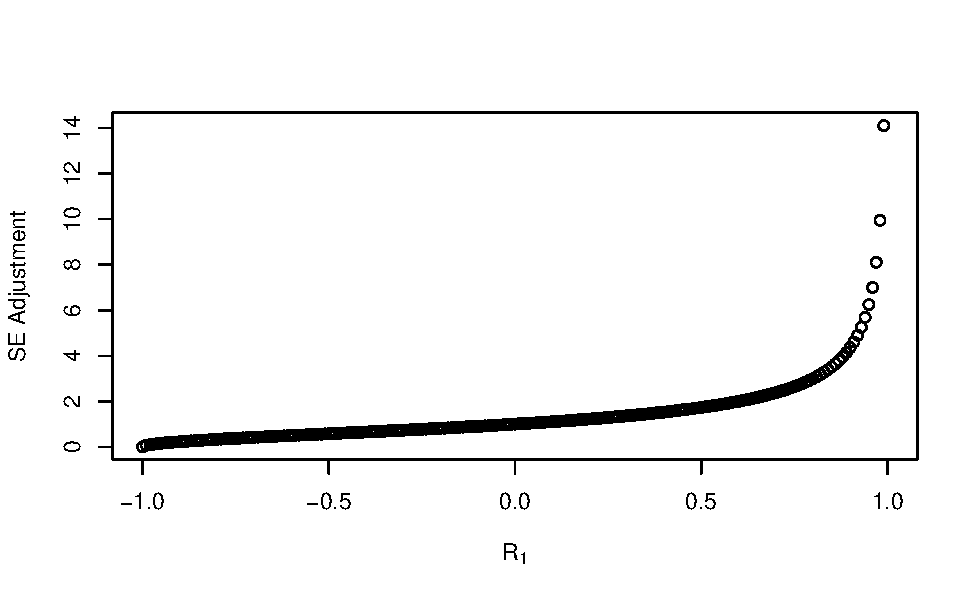
\includegraphics[width=\maxwidth]{figure/prob3b-1} 

}



\end{knitrout}

\item%3c
{\it This adjustment can also be used on the SEs from linear models to provided ``corrected" SEs for inference in the presence of autocorrelated errors. Since this is an approximation and performed after we complete our regular linear model analysis, we might want to see how it performs using a simulation study. For this simulation, consider three scenarios for the true process for our simulation study (white noise, AR(1), and MA(1)). Re-use the simulation setup from our previous homeworks (n=109 with Normal white noise with $\hat{\sigma^2_e}=0.03227^2$ and an AR(1) with $\phi=0.6$ that has the same variance). We need to generate an MA(1) process with similar variability as well. There is a complication in using ``arima.sim" for simulating MA(1) processes that we will discuss more later in terms of positive or negative signs on coefficients, but use ``arima.sim(n=109,list(ma=0.6),sd=sqrt(0.0007657007))" to simulate from $Y_t=e_t+0.6e_{t-1}$ with $\sigma^2_e=0.0007657007$ for generating a third response variable.}

\begin{knitrout}\footnotesize
\definecolor{shadecolor}{rgb}{1, 1, 1}\color{fgcolor}\begin{kframe}
\begin{alltt}
\hlkwd{set.seed}\hlstd{(}\hlnum{13567}\hlstd{)}
\hlstd{x}\hlkwb{<-}\hlnum{1901}\hlopt{:}\hlnum{2009}

\hlkwd{require}\hlstd{(nlme)}

\hlstd{Sims}\hlkwb{<-}\hlnum{1000}
\hlstd{ysimar1} \hlkwb{<-} \hlkwa{NULL}
\hlstd{ysimma1} \hlkwb{<-} \hlkwa{NULL}
\hlstd{ysimwn} \hlkwb{<-} \hlkwa{NULL}
\hlkwa{for} \hlstd{(k} \hlkwa{in} \hlstd{(}\hlnum{1}\hlopt{:}\hlstd{Sims))\{}
  \hlcom{#we are to use phi = 0.6 for ar1 with sd = 0.03227}
  \hlcom{#for the normal wn we are to use sd = 0.0322}
  \hlcom{#for ma1 we are to use ma = 0.6 and sd = 0.0007657007}
  \hlcom{#are these comparible with different sd's?}
\hlstd{ysimar1}\hlkwb{<-}\hlkwd{arima.sim}\hlstd{(}\hlkwc{n}\hlstd{=}\hlnum{109}\hlstd{,}\hlkwc{model}\hlstd{=}\hlkwd{list}\hlstd{(}\hlkwc{ar}\hlstd{=}\hlkwd{c}\hlstd{(}\hlnum{0.6}\hlstd{)),}\hlkwc{sd}\hlstd{=}\hlkwd{sqrt}\hlstd{(}\hlnum{0.03227}\hlstd{))}
\hlstd{ysimma1}\hlkwb{<-}\hlkwd{arima.sim}\hlstd{(}\hlkwc{n}\hlstd{=}\hlnum{109}\hlstd{,}\hlkwd{list}\hlstd{(}\hlkwc{ma}\hlstd{=}\hlnum{0.6}\hlstd{),}\hlkwc{sd}\hlstd{=}\hlkwd{sqrt}\hlstd{(}\hlnum{0.0007657007}\hlstd{))}
\hlstd{ysimwn}\hlkwb{<-}\hlkwd{rnorm}\hlstd{(}\hlkwc{n}\hlstd{=}\hlnum{109}\hlstd{,}\hlnum{0}\hlstd{,}\hlkwc{sd} \hlstd{=} \hlkwd{sqrt}\hlstd{(}\hlnum{0.03227}\hlstd{))}
\hlstd{\}}
\end{alltt}
\end{kframe}
\end{knitrout}

{\it Verify that the MA(1) process I provided has the correct variance of $0.03227^2$ with these settings based on checking its theoretical variance. Show your work. (5 pts)}

\begin{knitrout}\footnotesize
\definecolor{shadecolor}{rgb}{1, 1, 1}\color{fgcolor}\begin{kframe}
\begin{alltt}
\hlstd{var.ysimma1} \hlkwb{<-} \hlkwd{var}\hlstd{(ysimma1)}
\end{alltt}
\end{kframe}
\end{knitrout}

The correct variance is $0.03227^2$ = 0.0010414 and the simulated variance is very close at 0.0008956.

\item %3d
{\it Then for each of the three versions of the response, find the ``lm" slope for the trend and its SE to use in the adjustment and keep track the p-value for the regular slope t-test. To use the adjustment, we need to find the lag 1 SACF estimate which is available from ``acf(y,plot=F)\$acf[1]" (if you load ``TSA"). Use this value to correct the SE and then find a second p-value using the ``pt" function based on the ``corrected SE" and our regular t-test df. Report your code and the Type I error rates in these three scenarios for the regular ``lm" t-test and the t-tests with the corrected SEs (six different Type I error rates should be estimated but two we have already found in prior work). Discuss the success of the adjustment in the different situations based on your results. I am giving you a start to the needed code below for the white noise response part of the simulations. In my code, ``b1" needs to contain the estimated slope coefficient. (10 pts)}

\begin{kframe}
\begin{alltt}
\hlkwd{set.seed}\hlstd{(}\hlnum{13567}\hlstd{)}
\hlstd{x}\hlkwb{<-}\hlnum{1901}\hlopt{:}\hlnum{2009}

\hlstd{Sims}\hlkwb{<-}\hlnum{1000}
\hlstd{Pval_t}\hlkwb{<-}\hlstd{Pval_Corr}\hlkwb{<-}\hlkwd{matrix}\hlstd{(}\hlnum{NA}\hlstd{,}\hlkwc{nrow}\hlstd{=Sims)}
\hlstd{ysimwn}\hlkwb{<-}\hlkwd{replicate}\hlstd{(Sims,}\hlkwd{rnorm}\hlstd{(}\hlkwc{n}\hlstd{=}\hlnum{109}\hlstd{,}\hlkwc{sd}\hlstd{=}\hlnum{0.03227}\hlstd{))}
\hlstd{ysimwn} \hlkwb{<-} \hlkwd{t}\hlstd{(ysimwn)}
\hlstd{Placeholder1} \hlkwb{<-} \hlkwa{NULL}
\hlstd{Placeholder2} \hlkwb{<-} \hlkwa{NULL}
\hlstd{b1} \hlkwb{<-} \hlkwa{NULL}
\hlstd{SE_corrected} \hlkwb{<-} \hlkwa{NULL}

\hlkwa{for} \hlstd{(k} \hlkwa{in} \hlstd{(}\hlnum{1}\hlopt{:}\hlstd{Sims))\{}
\hlstd{Pval_t[k]}\hlkwb{<-}\hlkwd{summary}\hlstd{(}\hlkwd{lm}\hlstd{(ysimwn[k,]}\hlopt{~}\hlstd{x))}\hlopt{$}\hlstd{coef[}\hlnum{2}\hlstd{,}\hlnum{4}\hlstd{]}
\hlcom{#pull off the pvalue for the slope coefficient}
\hlstd{r1[k]}\hlkwb{<-}\hlstd{stats}\hlopt{::}\hlkwd{acf}\hlstd{(ysimwn[k,],}\hlkwc{plot}\hlstd{=F)}\hlopt{$}\hlstd{acf[}\hlnum{2}\hlstd{]}\hlcom{#calculate the adjustment}
\hlcom{#pull off the next acf since I am using the stats package}

\hlstd{Placeholder1[k]}\hlkwb{<-}\hlkwd{summary}\hlstd{(}\hlkwd{lm}\hlstd{(ysimwn[k,]}\hlopt{~}\hlstd{x))}\hlopt{$}\hlstd{coefficients[}\hlnum{2}\hlstd{,}\hlnum{1}\hlstd{]}
\hlstd{Placeholder2[k]}\hlkwb{<-}\hlstd{(}\hlkwd{sqrt}\hlstd{(r1[k]} \hlopt{+}\hlnum{1}\hlstd{)}\hlopt{/}\hlstd{(}\hlnum{1}\hlopt{-}\hlstd{r1[k]))}\hlopt{*}\hlkwd{summary}\hlstd{(}
  \hlkwd{lm}\hlstd{(ysimwn[k,]}\hlopt{~}\hlstd{x))}\hlopt{$}\hlstd{coefficients[}\hlnum{2}\hlstd{,}\hlnum{2}\hlstd{]}

\hlstd{b1[k]}\hlkwb{<-}\hlstd{Placeholder1[k]}
\hlcom{# You need to replace Placeholder1 with information }
\hlcom{# from lm() note:: estimate of the slope!}

\hlcom{#shouldn't correct in the WN case}
\hlstd{SE_corrected[k]}\hlkwb{<-}\hlstd{(Placeholder2[k])}
\hlcom{#You need to replace Placeholder2 with information from lm()}
\hlstd{Pval_Corr[k]}\hlkwb{<-}\hlkwd{pt}\hlstd{(}\hlkwd{abs}\hlstd{(b1[k]}\hlopt{/}\hlstd{SE_corrected[k]),}\hlkwc{df}\hlstd{=}\hlnum{107}\hlstd{,}\hlkwc{lower.tail}\hlstd{=F)}
\hlstd{\}}

\hlstd{wn.type1.lm} \hlkwb{<-} \hlkwd{length}\hlstd{(}\hlkwd{which}\hlstd{(Pval_t} \hlopt{<=} \hlnum{0.05}\hlstd{)} \hlopt{==} \hlnum{TRUE}\hlstd{)}\hlopt{/}\hlkwd{length}\hlstd{(Pval_t)}
\hlstd{wn.type1.adj} \hlkwb{<-} \hlkwd{length}\hlstd{(}\hlkwd{which}\hlstd{(Pval_Corr} \hlopt{<=} \hlnum{0.05}\hlstd{)} \hlopt{==} \hlnum{TRUE}\hlstd{)}\hlopt{/}\hlkwd{length}\hlstd{(Pval_Corr)}


\hlcom{## next up is ar1}
\hlcom{## use ysimar1 from above}
\hlkwd{set.seed}\hlstd{(}\hlnum{13567}\hlstd{)}
\hlstd{x}\hlkwb{<-}\hlnum{1901}\hlopt{:}\hlnum{2009}

\hlstd{Sims}\hlkwb{<-}\hlnum{1000}
\hlstd{Pval_t}\hlkwb{<-}\hlstd{Pval_Corr}\hlkwb{<-}\hlkwd{matrix}\hlstd{(}\hlnum{NA}\hlstd{,}\hlkwc{nrow}\hlstd{=Sims)}
\hlstd{ysimar1}\hlkwb{<-}\hlkwd{replicate}\hlstd{(Sims,}\hlkwd{arima.sim}\hlstd{(}\hlkwc{n}\hlstd{=}\hlnum{109}\hlstd{,}\hlkwc{model}\hlstd{=}\hlkwd{list}\hlstd{(}
  \hlkwc{ar}\hlstd{=}\hlkwd{c}\hlstd{(}\hlnum{0.6}\hlstd{)),}\hlkwc{sd}\hlstd{=}\hlkwd{sqrt}\hlstd{(}\hlnum{0.03227}\hlstd{)))}
\hlstd{ysimar1} \hlkwb{<-} \hlkwd{t}\hlstd{(ysimar1)}

\hlcom{#so 1000 rows and 109 columns}

\hlkwa{for} \hlstd{(k} \hlkwa{in} \hlstd{(}\hlnum{1}\hlopt{:}\hlstd{Sims))\{}
\hlstd{Pval_t[k]}\hlkwb{<-}\hlkwd{summary}\hlstd{(}\hlkwd{lm}\hlstd{(ysimar1[k,]}\hlopt{~}\hlstd{x))}\hlopt{$}\hlstd{coef[}\hlnum{2}\hlstd{,}\hlnum{4}\hlstd{]}
\hlcom{#pull off the pvalue for the slope coefficient}
\hlstd{r1[k]}\hlkwb{<-}\hlstd{stats}\hlopt{::}\hlkwd{acf}\hlstd{(ysimar1[k,],}\hlkwc{plot}\hlstd{=F)}\hlopt{$}\hlstd{acf[}\hlnum{2}\hlstd{]}\hlcom{#calculate the adjustment}
\hlcom{#pull off the next acf since I am using the stats package}

\hlstd{Placeholder1[k]}\hlkwb{<-}\hlkwd{summary}\hlstd{(}\hlkwd{lm}\hlstd{(ysimar1[k,]}\hlopt{~}\hlstd{x))}\hlopt{$}\hlstd{coefficients[}\hlnum{2}\hlstd{,}\hlnum{1}\hlstd{]}
\hlstd{Placeholder2[k]}\hlkwb{<-}\hlstd{(}\hlkwd{sqrt}\hlstd{(r1[k]} \hlopt{+}\hlnum{1}\hlstd{)}\hlopt{/}\hlstd{(}\hlnum{1}\hlopt{-}\hlstd{r1[k]))}\hlopt{*}\hlkwd{summary}\hlstd{(}
  \hlkwd{lm}\hlstd{(ysimar1[k,]}\hlopt{~}\hlstd{x))}\hlopt{$}\hlstd{coefficients[}\hlnum{2}\hlstd{,}\hlnum{2}\hlstd{]}

\hlstd{b1[k]}\hlkwb{<-}\hlstd{Placeholder1[k]}
\hlcom{# You need to replace Placeholder1 with information }
\hlcom{# from lm() note:: estimate of the slope!}

\hlcom{#i don't see why we are correcting the se in the WN case}
\hlstd{SE_corrected[k]}\hlkwb{<-}\hlstd{(Placeholder2[k])}
\hlcom{#You need to replace Placeholder2 with information from lm()}
\hlstd{Pval_Corr[k]}\hlkwb{<-}\hlkwd{pt}\hlstd{(}\hlkwd{abs}\hlstd{(b1[k]}\hlopt{/}\hlstd{SE_corrected[k]),}\hlkwc{df}\hlstd{=}\hlnum{107}\hlstd{,}\hlkwc{lower.tail}\hlstd{=F)}
\hlstd{\}}

\hlstd{ar1.type1.lm} \hlkwb{<-} \hlkwd{length}\hlstd{(}\hlkwd{which}\hlstd{(Pval_t} \hlopt{<=} \hlnum{0.05}\hlstd{)} \hlopt{==} \hlnum{TRUE}\hlstd{)}\hlopt{/}\hlkwd{length}\hlstd{(Pval_t)}
\hlstd{ar1.type1.adj} \hlkwb{<-} \hlkwd{length}\hlstd{(}\hlkwd{which}\hlstd{(Pval_Corr} \hlopt{<=} \hlnum{0.05}\hlstd{)} \hlopt{==} \hlnum{TRUE}\hlstd{)}\hlopt{/}\hlkwd{length}\hlstd{(Pval_Corr)}


\hlcom{## finally is ma1}
\hlcom{## use ysimma1 from above}
\hlkwd{set.seed}\hlstd{(}\hlnum{13567}\hlstd{)}
\hlstd{x}\hlkwb{<-}\hlnum{1901}\hlopt{:}\hlnum{2009}

\hlstd{Sims}\hlkwb{<-}\hlnum{1000}
\hlstd{Pval_t}\hlkwb{<-}\hlstd{Pval_Corr}\hlkwb{<-}\hlkwd{matrix}\hlstd{(}\hlnum{NA}\hlstd{,}\hlkwc{nrow}\hlstd{=Sims)}
\hlstd{ysimma1}\hlkwb{<-}\hlkwd{replicate}\hlstd{(Sims,}\hlkwd{arima.sim}\hlstd{(}\hlkwc{n}\hlstd{=}\hlnum{109}\hlstd{,}\hlkwd{list}\hlstd{(}
  \hlkwc{ma}\hlstd{=}\hlnum{0.6}\hlstd{),}\hlkwc{sd}\hlstd{=}\hlkwd{sqrt}\hlstd{(}\hlnum{0.0007657007}\hlstd{)))}
\hlstd{ysimma1} \hlkwb{<-} \hlkwd{t}\hlstd{(ysimma1)}

\hlcom{#so 1000 rows and 109 columns}

\hlkwa{for} \hlstd{(k} \hlkwa{in} \hlstd{(}\hlnum{1}\hlopt{:}\hlstd{Sims))\{}
\hlstd{Pval_t[k]}\hlkwb{<-}\hlkwd{summary}\hlstd{(}\hlkwd{lm}\hlstd{(ysimma1[k,]}\hlopt{~}\hlstd{x))}\hlopt{$}\hlstd{coef[}\hlnum{2}\hlstd{,}\hlnum{4}\hlstd{]}
\hlcom{#pull off the pvalue for the slope coefficient}
\hlstd{r1[k]}\hlkwb{<-}\hlstd{stats}\hlopt{::}\hlkwd{acf}\hlstd{(ysimma1[k,],}\hlkwc{plot}\hlstd{=F)}\hlopt{$}\hlstd{acf[}\hlnum{2}\hlstd{]}\hlcom{#calculate the adjustment}
\hlcom{#pull off the next acf since I am using the stats package}

\hlstd{Placeholder1[k]}\hlkwb{<-}\hlkwd{summary}\hlstd{(}\hlkwd{lm}\hlstd{(ysimma1[k,]}\hlopt{~}\hlstd{x))}\hlopt{$}\hlstd{coefficients[}\hlnum{2}\hlstd{,}\hlnum{1}\hlstd{]}
\hlstd{Placeholder2[k]}\hlkwb{<-}\hlstd{(}\hlkwd{sqrt}\hlstd{(r1[k]} \hlopt{+}\hlnum{1}\hlstd{)}\hlopt{/}\hlstd{(}\hlnum{1}\hlopt{-}\hlstd{r1[k]))}\hlopt{*}\hlkwd{summary}\hlstd{(}
  \hlkwd{lm}\hlstd{(ysimma1[k,]}\hlopt{~}\hlstd{x))}\hlopt{$}\hlstd{coefficients[}\hlnum{2}\hlstd{,}\hlnum{2}\hlstd{]}

\hlstd{b1[k]}\hlkwb{<-}\hlstd{Placeholder1[k]}
\hlcom{# You need to replace Placeholder1 with information}
\hlcom{# from lm() note:: estimate of the slope!}

\hlcom{#i don't see why we are correcting the se in the WN case}
\hlstd{SE_corrected[k]}\hlkwb{<-}\hlstd{(Placeholder2[k])}
\hlcom{#You need to replace Placeholder2 with information from lm()}
\hlstd{Pval_Corr[k]}\hlkwb{<-}\hlkwd{pt}\hlstd{(}\hlkwd{abs}\hlstd{(b1[k]}\hlopt{/}\hlstd{SE_corrected[k]),}\hlkwc{df}\hlstd{=}\hlnum{107}\hlstd{,}\hlkwc{lower.tail}\hlstd{=F)}
\hlstd{\}}

\hlstd{ma1.type1.lm} \hlkwb{<-} \hlkwd{length}\hlstd{(}\hlkwd{which}\hlstd{(Pval_t} \hlopt{<=} \hlnum{0.05}\hlstd{)} \hlopt{==} \hlnum{TRUE}\hlstd{)}\hlopt{/}\hlkwd{length}\hlstd{(Pval_t)}
\hlstd{ma1.type1.adj} \hlkwb{<-} \hlkwd{length}\hlstd{(}\hlkwd{which}\hlstd{(Pval_Corr} \hlopt{<=} \hlnum{0.05}\hlstd{)} \hlopt{==} \hlnum{TRUE}\hlstd{)}\hlopt{/}\hlkwd{length}\hlstd{(Pval_Corr)}

\hlcom{#You need to write two more similar loops and then calculate estimated Type I error rates}

\hlcom{#I'm guessing the two other }

\hlstd{tb.pvalues} \hlkwb{<-} \hlkwd{matrix}\hlstd{(}\hlkwd{c}\hlstd{(wn.type1.lm,wn.type1.adj,ar1.type1.lm,}
                       \hlstd{ar1.type1.adj,ma1.type1.lm,ma1.type1.adj),} \hlkwc{nrow} \hlstd{=} \hlnum{3}\hlstd{,}
                     \hlkwc{ncol} \hlstd{=} \hlnum{2}\hlstd{,} \hlkwc{byrow} \hlstd{=} \hlnum{TRUE}\hlstd{)}
\hlkwd{colnames}\hlstd{(tb.pvalues)} \hlkwb{<-} \hlkwd{c}\hlstd{(}\hlstr{"LM pvalue"}\hlstd{,} \hlstr{"Adj. pvalue"}\hlstd{)}
\hlkwd{rownames}\hlstd{(tb.pvalues)} \hlkwb{<-} \hlkwd{c}\hlstd{(}\hlstr{"WN"}\hlstd{,} \hlstr{"AR1"}\hlstd{,} \hlstr{"MA1"}\hlstd{)}

\hlkwd{print}\hlstd{(}\hlkwd{xtable}\hlstd{(tb.pvalues,} \hlkwc{align} \hlstd{=} \hlstr{"||r|r|r||"}\hlstd{,} \hlkwc{digits} \hlstd{=} \hlnum{3}\hlstd{))}
\end{alltt}
\end{kframe}% latex table generated in R 3.3.1 by xtable 1.8-2 package
% Wed Nov 09 15:18:11 2016
\begin{table}[H]
\centering
\begin{tabular}{||r|r|r||}
  \hline
 & LM pvalue & Adj. pvalue \\ 
  \hline
WN & 0.047 & 0.106 \\ 
  AR1 & 0.343 & 0.018 \\ 
  MA1 & 0.173 & 0.009 \\ 
   \hline
\end{tabular}
\end{table}


In the WN process, we should not need to adjust for correlated errors, and so it is not surprising that the adjusted pvalue is too large and that the unadjusted pvalue is near the 0.05 specified type I error rate.

The LM pvalues, or the unadjusted pvalues are too small, resulting in too many ``significant" slope terms (34.3\% of the AR1 pvalues are $\leq $ 0.05 and 17.3\% of the MA1 pvalues are). However, the adjustment seems to adjust too much. We would expect to reject roughly 5\% of the time by random chance, but we are rejecting around 2\% of the time for the AR1 process and 1\% roughly for the MA1 process with the adjustment.

\end{enumerate}

\item%4

\begin{knitrout}\footnotesize
\definecolor{shadecolor}{rgb}{1, 1, 1}\color{fgcolor}\begin{kframe}
\begin{alltt}
\hlstd{Bozeman} \hlkwb{<-} \hlkwd{read.csv}\hlstd{(}\hlstr{"Bozeman.csv"}\hlstd{,} \hlkwc{as.is} \hlstd{=} \hlnum{TRUE}\hlstd{)}

\hlstd{monthsF}\hlkwb{<-}\hlkwd{sort}\hlstd{(}\hlkwd{unique}\hlstd{(Bozeman}\hlopt{$}\hlstd{MonthRE))}
\hlstd{countfun}\hlkwb{<-}\hlkwa{function}\hlstd{(}\hlkwc{x}\hlstd{)} \hlkwd{c}\hlstd{(}\hlkwd{sum}\hlstd{(x}\hlopt{<}\hlnum{32}\hlstd{),}\hlkwd{sum}\hlstd{(}\hlopt{!}\hlkwd{is.na}\hlstd{(x)))}

\hlstd{monthcountMINF}\hlkwb{<-}\hlkwd{aggregate}\hlstd{(Bozeman}\hlopt{$}\hlstd{TMIN..F.,}
                          \hlkwc{by}\hlstd{=}\hlkwd{list}\hlstd{(Bozeman}\hlopt{$}\hlstd{MonthRE),}\hlkwc{FUN}\hlstd{=countfun)}
\hlstd{yearcountMINF}\hlkwb{<-}\hlkwd{aggregate}\hlstd{(Bozeman}\hlopt{$}\hlstd{TMIN..F.,}
                         \hlkwc{by}\hlstd{=}\hlkwd{list}\hlstd{(Bozeman}\hlopt{$}\hlstd{Year),}\hlkwc{FUN}\hlstd{=countfun)}

\hlstd{bz}\hlkwb{<-}\hlkwd{data.frame}\hlstd{(}\hlkwc{Year}\hlstd{=yearcountMINF[,}\hlnum{1}\hlstd{],}
               \hlkwc{DaysBelow32}\hlstd{=yearcountMINF}\hlopt{$}\hlstd{x[,}\hlnum{1}\hlstd{],}
                  \hlkwc{MeasuredDays}\hlstd{=yearcountMINF}\hlopt{$}\hlstd{x[,}\hlnum{2}\hlstd{],}
                  \hlkwc{PropDays}\hlstd{=yearcountMINF}\hlopt{$}\hlstd{x[,}\hlnum{1}\hlstd{]}\hlopt{/}\hlstd{yearcountMINF}\hlopt{$}\hlstd{x[,}\hlnum{2}\hlstd{])}

\hlcom{#head(bz)}
\end{alltt}
\end{kframe}
\end{knitrout}

\begin{knitrout}\footnotesize
\definecolor{shadecolor}{rgb}{1, 1, 1}\color{fgcolor}\begin{kframe}
\begin{alltt}
\hlstd{bz}\hlopt{$}\hlstd{logitPropDays} \hlkwb{<-} \hlstd{mosaic}\hlopt{::}\hlkwd{logit}\hlstd{(bz}\hlopt{$}\hlstd{PropDays)}
\end{alltt}
\end{kframe}
\end{knitrout}

\begin{enumerate}
\item%4a
{\it With the logit of the proportion response variable as your response variable, use AIC comparisons to identify the form of the polynomial trend (linear, quadratic, or cubic) and whether you benefit from including AR(1) and MA(1) correlations using GLS models. Select across all these possible combinations including not having autocorrelation or a trend using AICs and discuss all aspects of that result. Remember to use `ML` estimation for all comparisons since the fixed effects vary across the models being compared. Discuss the strength of support for the top selected model(s). (10 pts)}

\begin{kframe}
\begin{alltt}
\hlstd{glsl} \hlkwb{<-} \hlkwd{gls}\hlstd{(logitPropDays} \hlopt{~} \hlstd{Year,} \hlkwc{data} \hlstd{= bz,} \hlkwc{method} \hlstd{=} \hlstr{"ML"}\hlstd{)}
\hlstd{glsq} \hlkwb{<-} \hlkwd{gls}\hlstd{(logitPropDays} \hlopt{~} \hlkwd{poly}\hlstd{(Year,}\hlnum{2}\hlstd{),} \hlkwc{data} \hlstd{= bz,} \hlkwc{method} \hlstd{=} \hlstr{"ML"}\hlstd{)}
\hlstd{glscube} \hlkwb{<-} \hlkwd{gls}\hlstd{(logitPropDays} \hlopt{~} \hlkwd{poly}\hlstd{(Year,} \hlnum{3}\hlstd{),} \hlkwc{data} \hlstd{= bz,} \hlkwc{method} \hlstd{=} \hlstr{"ML"}\hlstd{)}

\hlcom{#p = ar1; q = ma}
\hlstd{glsl.ar1} \hlkwb{<-} \hlkwd{gls}\hlstd{(logitPropDays} \hlopt{~} \hlstd{Year,} \hlkwc{data} \hlstd{= bz,}
                \hlkwc{correlation}\hlstd{=}\hlkwd{corARMA}\hlstd{(}\hlkwc{p}\hlstd{=}\hlnum{1}\hlstd{,}\hlkwc{q}\hlstd{=}\hlnum{0}\hlstd{),}\hlkwc{method}\hlstd{=}\hlstr{"ML"}\hlstd{)}
\hlstd{glsq.ar1} \hlkwb{<-} \hlkwd{gls}\hlstd{(logitPropDays} \hlopt{~} \hlkwd{poly}\hlstd{(Year,} \hlnum{2}\hlstd{),} \hlkwc{data} \hlstd{= bz,}
                \hlkwc{correlation}\hlstd{=}\hlkwd{corARMA}\hlstd{(}\hlkwc{p}\hlstd{=}\hlnum{1}\hlstd{,}\hlkwc{q}\hlstd{=}\hlnum{0}\hlstd{),}\hlkwc{method}\hlstd{=}\hlstr{"ML"}\hlstd{)}
\hlstd{glscube.ar1} \hlkwb{<-} \hlkwd{gls}\hlstd{(logitPropDays} \hlopt{~} \hlkwd{poly}\hlstd{(Year,}\hlnum{3}\hlstd{),} \hlkwc{data} \hlstd{= bz,}
                   \hlkwc{correlation}\hlstd{=}\hlkwd{corARMA}\hlstd{(}\hlkwc{p}\hlstd{=}\hlnum{1}\hlstd{,}\hlkwc{q}\hlstd{=}\hlnum{0}\hlstd{),}\hlkwc{method}\hlstd{=}\hlstr{"ML"}\hlstd{)}


\hlstd{glsl.ma} \hlkwb{<-} \hlkwd{gls}\hlstd{(logitPropDays} \hlopt{~} \hlstd{Year,} \hlkwc{data} \hlstd{= bz,}
               \hlkwc{correlation}\hlstd{=}\hlkwd{corARMA}\hlstd{(}\hlkwc{p}\hlstd{=}\hlnum{0}\hlstd{,}\hlkwc{q}\hlstd{=}\hlnum{1}\hlstd{),}\hlkwc{method}\hlstd{=}\hlstr{"ML"}\hlstd{)}
\hlstd{glsq.ma} \hlkwb{<-} \hlkwd{gls}\hlstd{(logitPropDays} \hlopt{~} \hlkwd{poly}\hlstd{(Year,} \hlnum{2}\hlstd{),} \hlkwc{data} \hlstd{= bz,}
               \hlkwc{correlation}\hlstd{=}\hlkwd{corARMA}\hlstd{(}\hlkwc{p}\hlstd{=}\hlnum{0}\hlstd{,}\hlkwc{q}\hlstd{=}\hlnum{1}\hlstd{),}\hlkwc{method}\hlstd{=}\hlstr{"ML"}\hlstd{)}
\hlstd{glscube.ma} \hlkwb{<-} \hlkwd{gls}\hlstd{(logitPropDays} \hlopt{~} \hlkwd{poly}\hlstd{(Year,}\hlnum{3}\hlstd{),} \hlkwc{data} \hlstd{= bz,}
                  \hlkwc{correlation}\hlstd{=}\hlkwd{corARMA}\hlstd{(}\hlkwc{p}\hlstd{=}\hlnum{0}\hlstd{,}\hlkwc{q}\hlstd{=}\hlnum{1}\hlstd{),}\hlkwc{method}\hlstd{=}\hlstr{"ML"}\hlstd{)}


\hlstd{gls.aic} \hlkwb{<-} \hlkwd{AIC}\hlstd{(glsl, glsq, glscube, glsl.ar1, glsq.ar1,}
               \hlstd{glscube.ar1, glsl.ma, glsq.ma, glscube.ma)}
\hlstd{gls.aic} \hlkwb{<-} \hlstd{gls.aic[}\hlkwd{with}\hlstd{(gls.aic,} \hlkwd{order}\hlstd{(AIC)), ]}

\hlkwd{print}\hlstd{(}\hlkwd{xtable}\hlstd{(gls.aic))}
\end{alltt}
\end{kframe}% latex table generated in R 3.3.1 by xtable 1.8-2 package
% Wed Nov 09 15:18:13 2016
\begin{table}[H]
\centering
\begin{tabular}{rrr}
  \hline
 & df & AIC \\ 
  \hline
glsl.ar1 & 4.00 & -137.92 \\ 
  glsl.ma & 4.00 & -137.03 \\ 
  glsq.ar1 & 5.00 & -136.04 \\ 
  glsq.ma & 5.00 & -135.23 \\ 
  glscube.ar1 & 6.00 & -134.65 \\ 
  glscube.ma & 6.00 & -133.80 \\ 
  glsl & 3.00 & -131.36 \\ 
  glsq & 4.00 & -129.72 \\ 
  glscube & 5.00 & -128.20 \\ 
   \hline
\end{tabular}
\end{table}
\begin{kframe}\begin{alltt}
\hlcom{#this gives an error, but returns the exact same aic's found without error }
\end{alltt}
\end{kframe}

The logit response with an AR1 correlation structure fit with a linear long term trend model had 4 free degrees of freedom and the lowest AIC of -137.9151. Both having 4 free degrees of freedom and roughly 0.9 difference in AIC, there is weak evidence for the logit AR1 linear long term trend model relative to the logit MA1 linear long term trend model. 

Preference in terms of covariance structure is highest for the AR1, next highest for the MA1, and lowest for no induced covariance structure. Within each considered covariance structure, linear models are preferred, followed by quadratic and cubic long term trends sequentially. Linear models with AR1 and MA1 covariance structures have 4 free degrees of freedom, and the free degrees of freedom increases by 1 for each additional long term order added for the AR1 and MA1 models.

Focusing on models with induced correlation structures, the increase in AIC is not substantial AR1 and MA1 within a given order of the long term trend. Within each order of long term trend model, AR1 is preferred to MA1, but again the drop in AIC is minimal with the same free degrees of freedom. This makes for some preference for the linear model with an induced correlation structure relative to such quadratic models with more preference for linear models with induced correlation structures than the quadratic counterparts. For example, the linear AR1 and MA1 models have 4 free degrees of freedom and AICs of -137.9151 and -137.0275 respectively. These models only have 1 less free parameter and a drop of 1 to 2 AIC units relative to the quadratic AR1 and MA counterparts. Changes in free degrees of freedom and changes in AICs can be made between all pairwise long term trend models with the same induced correlation structures could similarly be compared. Note that I am referring to induced correlation structures as specifying AR1 or MA1 proccesses when fitting models. There is strong preference for linear models with induced correlation structures relative to cubic models with induced correlation structures and also in relation to all models fit without induced correlation structures with drops in AIC larger than 2 for each additional free parameter.

Again, within each long term trend category in models with specified correlation structures, AR1 correlation structures are slightly preferred to moving average structures.


\item%4b
{\it For your top AIC model, discuss the estimated total change over the entire data set, providing an ``effects" plot to support the discussion. You can keep the interpretation on the logit (log-odds)  scale. Support that discussion with either a t-test or an ANOVA F-test for the trend component that is fully reported and interpreted in a single sentence. [Ignore the fact that you selected this model using AICs in reporting the test result.] (6 pts)
}

\begin{knitrout}\footnotesize
\definecolor{shadecolor}{rgb}{1, 1, 1}\color{fgcolor}\begin{kframe}
\begin{alltt}
\hlkwd{plot}\hlstd{(}\hlkwd{allEffects}\hlstd{(glsl.ar1))}
\end{alltt}
\end{kframe}

{\centering 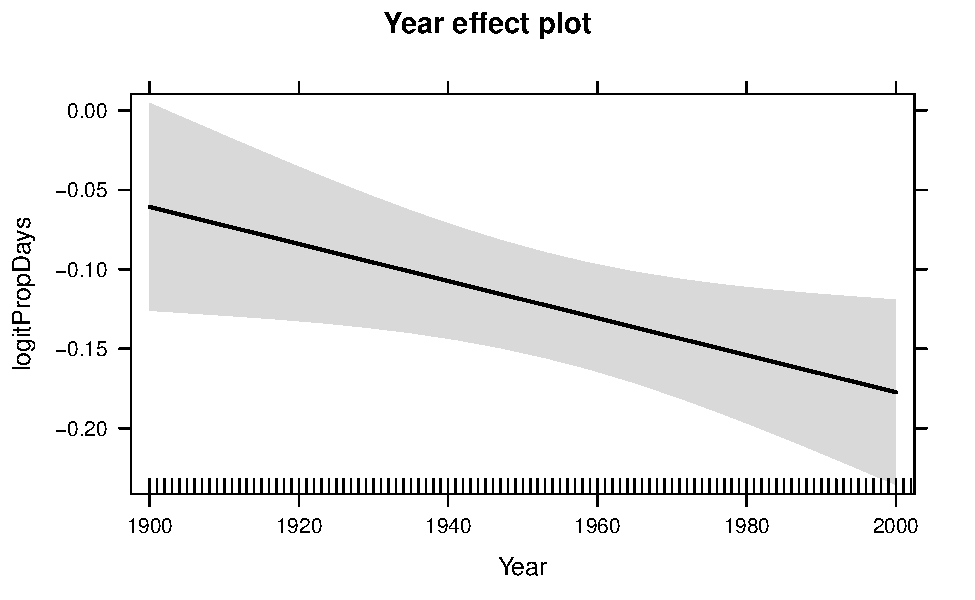
\includegraphics[width=\maxwidth]{figure/prob4b-1} 

}


\begin{kframe}\begin{alltt}
\hlstd{car}\hlopt{::}\hlkwd{Anova}\hlstd{(glsl.ar1,} \hlkwc{type} \hlstd{=} \hlstr{"II"}\hlstd{)}
\end{alltt}
\begin{verbatim}
Analysis of Deviance Table (Type II tests)

Response: logitPropDays
     Df  Chisq Pr(>Chisq)
Year  1 4.9329    0.02635
\end{verbatim}
\end{kframe}
\end{knitrout}

Data started being recorded in 1900 and the final year was 2008, 108 years total. On average, the logit proportion of days below freezing is estimated to have decreased by -0.0012*108 = -0.1296 with some variation. The effects plot shows a clear negative linear trend in the logit proportion of days below freezing as time progressed.

Based on a $\chi^2_{1df}$ test statistic, a (one-sided) pvalue of 0.02635 provides some evidence that the that the logit proportion of days below freezing decreased between 1900 and 2008 in relevant sampling areas of Bozeman, MT.
\end{enumerate}

\item %5 electricity  in austrailia
\begin{knitrout}\footnotesize
\definecolor{shadecolor}{rgb}{1, 1, 1}\color{fgcolor}\begin{kframe}
\begin{alltt}
\hlcom{#require(stR)}
\hlcom{#data(electricity,package="stR") #Note: Day 0 = January 10, 2000 was a Monday, first observation at time 00:00=midnight}

\hlcom{#Elec1<-data.frame(Demand=as.vector(electricity[,1]),}
                  \hlcom{#Time=as.vector(electricity[,3]),Day=}
                    \hlcom{#floor(as.vector(electricity[,3])/48),DayofWeek=}
                    \hlcom{#c(rep(rep(0:6,each=48),16),rep(0:2,each=48))/7,}
                  \hlcom{#TimeofDay=as.vector(electricity[,4])/48)}
\hlstd{Elec1} \hlkwb{<-} \hlkwd{read.csv}\hlstd{(}\hlstr{"Elec1.csv"}\hlstd{,} \hlkwc{header} \hlstd{=} \hlnum{TRUE}\hlstd{)}

\hlstd{Elec1}\hlopt{$}\hlstd{Dayfrac}\hlkwb{<-}\hlstd{Elec1}\hlopt{$}\hlstd{Day}\hlopt{+}\hlstd{Elec1}\hlopt{$}\hlstd{TimeofDay}
\hlstd{Elec1}\hlopt{$}\hlstd{DayofWeekF}\hlkwb{<-}\hlkwd{factor}\hlstd{(Elec1}\hlopt{$}\hlstd{DayofWeek)}
\hlstd{Elec1}\hlopt{$}\hlstd{TimeofDayF}\hlkwb{<-}\hlkwd{factor}\hlstd{(Elec1}\hlopt{$}\hlstd{TimeofDay)}

\hlstd{m1}\hlkwb{<-}\hlkwd{lm}\hlstd{(Demand}\hlopt{~}\hlstd{Dayfrac}\hlopt{+}\hlstd{DayofWeekF}\hlopt{+}\hlstd{TimeofDayF,}\hlkwc{data}\hlstd{=Elec1)}
\end{alltt}
\end{kframe}
\end{knitrout}
\begin{enumerate}
\item %5a

{\it Make a nice time series plot of the electricity demand. You can plot this using days since January 10, 2000 on the x-axis but you can get a bonus if you get dates to appear on the axis labels. I don't have details on the units of electicity consumption but lets suppose they are in total Watts consumed per 1000 people in 30 minutes. Discuss patterns in the long term mean energy consumption over this data set, potential seasonality (two kinds), and the potential for changing variability and outliers based only on the plot over time. (6 pts)}
\begin{knitrout}\footnotesize
\definecolor{shadecolor}{rgb}{1, 1, 1}\color{fgcolor}\begin{kframe}
\begin{alltt}
\hlstd{Elec1}\hlopt{$}\hlstd{time.expanded} \hlkwb{<-} \hlkwd{as.factor}\hlstd{(}\hlkwd{as.character}\hlstd{(}\hlkwd{weekdays}\hlstd{(}
  \hlkwd{as.Date}\hlstd{(Elec1}\hlopt{$}\hlstd{Time,} \hlkwc{origin} \hlstd{=} \hlstr{"2000-01-10"}\hlstd{))))}
\hlstd{Elec1}\hlopt{$}\hlstd{time.expanded} \hlkwb{<-} \hlkwd{substr}\hlstd{(Elec1}\hlopt{$}\hlstd{time.expanded,}\hlnum{1}\hlstd{,}\hlnum{7}\hlstd{)}

\hlstd{x.breaks} \hlkwb{<-} \hlkwd{c}\hlstd{(}\hlkwd{seq}\hlstd{(}\hlnum{0}\hlstd{,}\hlnum{5520}\hlstd{,}\hlkwc{by} \hlstd{=} \hlnum{240}\hlstd{))}

\hlstd{h} \hlkwb{<-} \hlkwd{c}\hlstd{(}\hlnum{1}\hlopt{:}\hlnum{23}\hlstd{)}
\hlstd{day.names} \hlkwb{<-} \hlkwd{as.Date}\hlstd{(h,} \hlkwc{origin} \hlstd{=} \hlstr{"2000-01-10"}\hlstd{)}

\hlcom{#now only pull every other day}
\hlstd{even.elements} \hlkwb{<-} \hlkwd{c}\hlstd{(}\hlnum{0}\hlstd{,}\hlnum{2}\hlstd{,}\hlnum{4}\hlstd{,}\hlnum{6}\hlstd{,}\hlnum{8}\hlstd{,}\hlnum{10}\hlstd{,}\hlnum{12}\hlstd{,}\hlnum{14}\hlstd{,}\hlnum{16}\hlstd{,}\hlnum{18}\hlstd{,}\hlnum{20}\hlstd{,}\hlnum{22}\hlstd{)}

\hlstd{day.names.even} \hlkwb{<-} \hlstd{day.names[even.elements]}

\hlstd{day.names1} \hlkwb{<-} \hlkwd{substr}\hlstd{(day.names.even,}\hlnum{7}\hlstd{,}\hlnum{10}\hlstd{)}
\hlstd{day.names1} \hlkwb{<-} \hlkwd{as.factor}\hlstd{(}\hlkwd{as.character}\hlstd{(day.names1))}



\hlkwd{ggplot}\hlstd{(}\hlkwc{data} \hlstd{= Elec1,} \hlkwd{aes}\hlstd{(}\hlkwc{x} \hlstd{=} \hlkwd{time}\hlstd{(time.expanded),} \hlkwc{y} \hlstd{= Demand))} \hlopt{+}
  \hlkwd{theme}\hlstd{(}\hlkwc{axis.text.x}  \hlstd{=} \hlkwd{element_text}\hlstd{(}\hlkwc{angle}\hlstd{=}\hlnum{45}\hlstd{,} \hlkwc{vjust}\hlstd{=}\hlnum{10}\hlstd{,} \hlkwc{size}\hlstd{=}\hlnum{0.5}\hlstd{))} \hlopt{+}
  \hlkwd{geom_line}\hlstd{()} \hlopt{+} \hlkwd{scale_x_continuous}\hlstd{(}\hlstr{"Day in 2000"}\hlstd{,} \hlkwc{breaks} \hlstd{=}
    \hlkwd{c}\hlstd{(}\hlkwd{time}\hlstd{(Elec1}\hlopt{$}\hlstd{time.expanded)[x.breaks[even.elements}\hlopt{+}\hlnum{1}\hlstd{]]),} \hlkwc{labels} \hlstd{=}
      \hlstd{day.names1)} \hlopt{+}
  \hlkwd{ylab}\hlstd{(}\hlstr{"total Watts consumed per 1000 people in 30 minutes"}\hlstd{)} \hlopt{+} \hlkwd{theme_bw}\hlstd{()}
\end{alltt}
\end{kframe}

{\centering 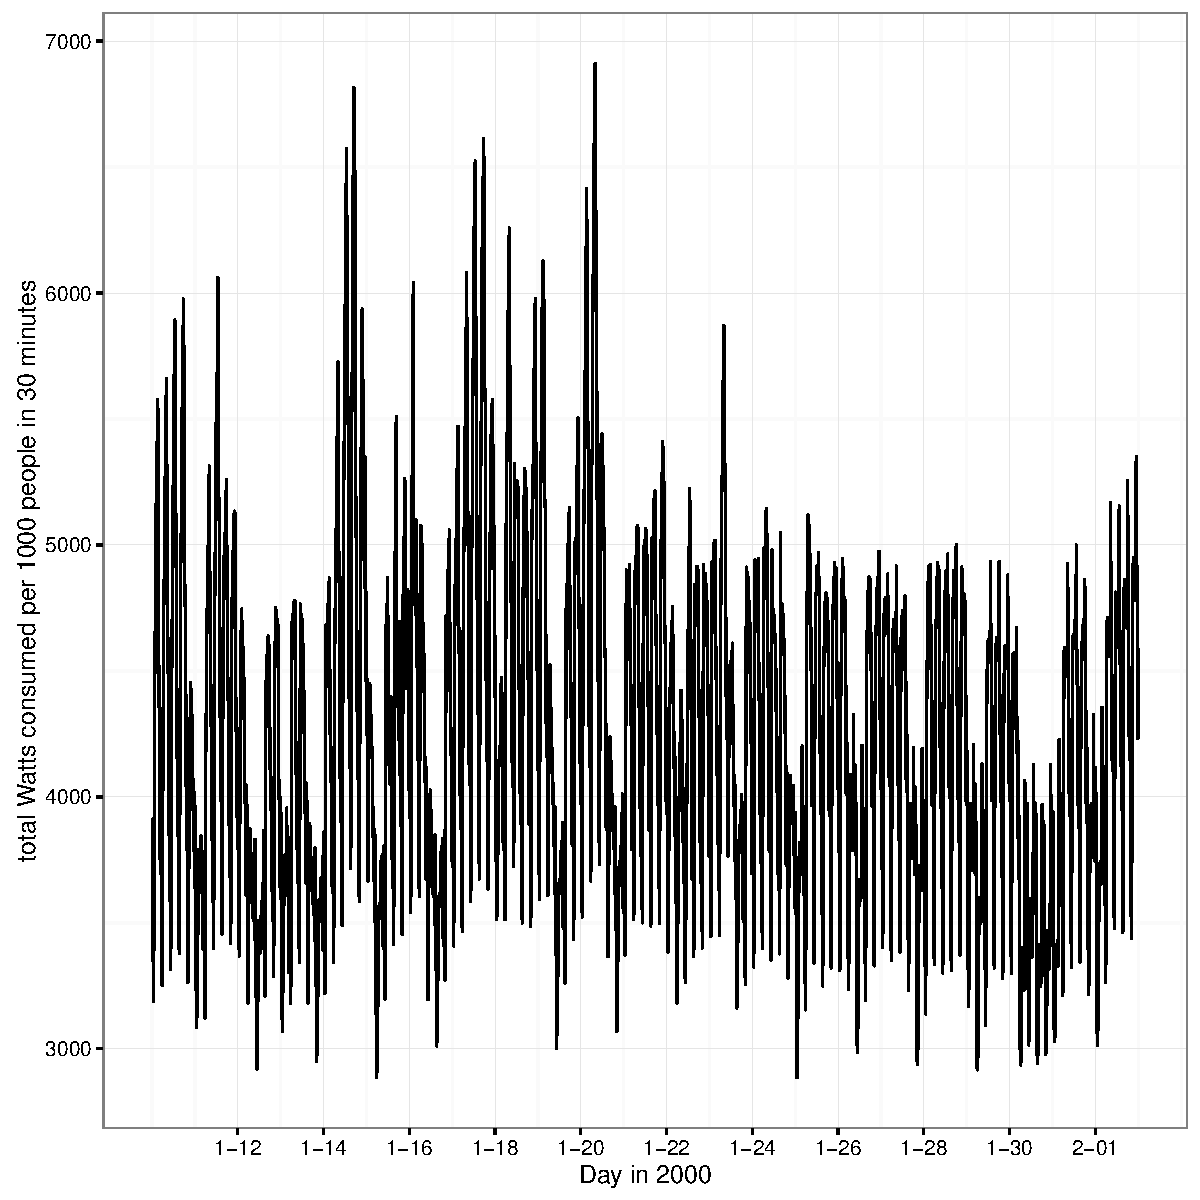
\includegraphics[width=\maxwidth]{figure/prob5a-1} 

}


\begin{kframe}\begin{alltt}
\hlcom{#the exact dates were too messy}
\end{alltt}
\end{kframe}
\end{knitrout}

{\bf Long Term Trends}

The long term mean trend appears to be fairly constant throughout the 30 minute increments sampled. The mean trend appears to have decreased slightly in 30 minute increments on January 13th and 14th, increased in 30 minute increments between the 5th and 10th days, so January 15 - January 20 and then slightly decreased again. The average long term total consumption then drops slightly, reaching it's low in this window on January 31st and then rises slightly again. Trends are Otherwise, throughout the entire time series, the long term trend appears to be fairly constant when considering all 30 minute increments sampled together.

\newpage

{\bf Seasonality}

In terms of days of the week (Monday, Tuesday, etc.) the drop in total consumption after the 23rd and fairly constant total consumption among days thereafter makes it difficult to pick up on day of the week trend since any pattern seen before the 23rd is discounted after that day. It appears the subsequent days have similar trends in total Watts consumed per 1000 people in 30 minutes, or that days show positive autocorrelation.  For example, consumption on January 10, 2000 is followed by a similar consuption on January 11 of 2000.

Within days, there appears to be a few consecutive 30 minute increments of low total consumption (most likely between 12:00 AM and 4:00 AM). This time of day seasonality is quite consistent throughout the entire time series.

\item%5b
{\it Use the provided model called ``m1" to generate tests for a linear trend, day of week, and time of day. Report the necessary test results in three sentences, one for each component. (8 pts) }

{\tiny
\begin{knitrout}\footnotesize
\definecolor{shadecolor}{rgb}{1, 1, 1}\color{fgcolor}\begin{kframe}
\begin{alltt}
\hlkwd{summary}\hlstd{(m1)}
\end{alltt}
\begin{verbatim}

Call:
lm(formula = Demand ~ Dayfrac + DayofWeekF + TimeofDayF, data = Elec1)

Residuals:
    Min      1Q  Median      3Q     Max 
-1600.6  -253.4   -35.1   231.8  1828.9 

Coefficients:
                       Estimate Std. Error t value Pr(>|t|)
(Intercept)           4327.3699    43.5653  99.331  < 2e-16
Dayfrac                 -2.7473     0.1745 -15.744  < 2e-16
DayofWeekF0.142857143   73.6320    21.2979   3.457 0.000550
DayofWeekF0.285714286  207.9701    21.3000   9.764  < 2e-16
DayofWeekF0.428571429   94.2447    21.6275   4.358 1.34e-05
DayofWeekF0.571428571 -482.7072    21.6275 -22.319  < 2e-16
DayofWeekF0.714285714 -804.4143    21.6290 -37.192  < 2e-16
DayofWeekF0.857142857 -125.0967    21.6318  -5.783 7.74e-09
TimeofDayF0.020833333 -160.7333    56.7307  -2.833 0.004624
TimeofDayF0.041666667   74.0662    56.7307   1.306 0.191752
TimeofDayF0.0625       -52.2379    56.7307  -0.921 0.357193
TimeofDayF0.083333333 -261.8003    56.7307  -4.615 4.02e-06
TimeofDayF0.104166667 -451.9592    56.7307  -7.967 1.97e-15
TimeofDayF0.125       -584.5277    56.7307 -10.304  < 2e-16
TimeofDayF0.145833333 -664.9948    56.7307 -11.722  < 2e-16
TimeofDayF0.166666667 -677.1425    56.7307 -11.936  < 2e-16
TimeofDayF0.1875      -633.4754    56.7307 -11.166  < 2e-16
TimeofDayF0.208333333 -473.9384    56.7307  -8.354  < 2e-16
TimeofDayF0.229166667 -291.0624    56.7307  -5.131 2.99e-07
TimeofDayF0.25          -6.2476    56.7307  -0.110 0.912313
TimeofDayF0.270833333  224.1657    56.7307   3.951 7.87e-05
TimeofDayF0.291666667  213.2391    56.7307   3.759 0.000173
TimeofDayF0.3125       306.4767    56.7307   5.402 6.86e-08
TimeofDayF0.333333333  408.1793    56.7307   7.195 7.09e-13
TimeofDayF0.354166667  464.5951    56.7307   8.189 3.24e-16
TimeofDayF0.375        525.4988    56.7307   9.263  < 2e-16
TimeofDayF0.395833333  568.2298    56.7307  10.016  < 2e-16
TimeofDayF0.416666667  610.5045    56.7307  10.761  < 2e-16
TimeofDayF0.4375       646.0620    56.7307  11.388  < 2e-16
TimeofDayF0.458333333  661.0063    56.7307  11.652  < 2e-16
TimeofDayF0.479166667  672.0874    56.7307  11.847  < 2e-16
TimeofDayF0.5          667.7155    56.7307  11.770  < 2e-16
TimeofDayF0.520833333  668.4612    56.7307  11.783  < 2e-16
TimeofDayF0.541666667  683.4800    56.7307  12.048  < 2e-16
TimeofDayF0.5625       678.6015    56.7308  11.962  < 2e-16
TimeofDayF0.583333333  665.4737    56.7308  11.730  < 2e-16
TimeofDayF0.604166667  665.2761    56.7308  11.727  < 2e-16
TimeofDayF0.625        676.3118    56.7308  11.921  < 2e-16
TimeofDayF0.645833333  690.0798    56.7308  12.164  < 2e-16
TimeofDayF0.666666667  688.1247    56.7308  12.130  < 2e-16
TimeofDayF0.6875       674.3220    56.7308  11.886  < 2e-16
TimeofDayF0.708333333  605.5723    56.7308  10.674  < 2e-16
TimeofDayF0.729166667  560.6935    56.7308   9.883  < 2e-16
TimeofDayF0.75         528.1999    56.7308   9.311  < 2e-16
TimeofDayF0.770833333  495.1622    56.7308   8.728  < 2e-16
TimeofDayF0.791666667  449.4590    56.7308   7.923 2.80e-15
TimeofDayF0.8125       427.4564    56.7308   7.535 5.69e-14
TimeofDayF0.833333333  353.5797    56.7309   6.233 4.93e-10
TimeofDayF0.854166667  246.4757    56.7309   4.345 1.42e-05
TimeofDayF0.875         97.7868    56.7309   1.724 0.084819
TimeofDayF0.895833333  -46.3870    56.7309  -0.818 0.413583
TimeofDayF0.916666667 -134.2602    56.7309  -2.367 0.017986
TimeofDayF0.9375      -181.4841    56.7309  -3.199 0.001387
TimeofDayF0.958333333  197.7191    56.7309   3.485 0.000496
TimeofDayF0.979166667  170.1108    56.7309   2.999 0.002725

Residual standard error: 430.2 on 5465 degrees of freedom
Multiple R-squared:  0.6237,	Adjusted R-squared:   0.62 
F-statistic: 167.7 on 54 and 5465 DF,  p-value: < 2.2e-16
\end{verbatim}
\begin{alltt}
\hlstd{car}\hlopt{::}\hlkwd{Anova}\hlstd{(m1,} \hlkwc{type} \hlstd{=} \hlstr{"II"}\hlstd{)}
\end{alltt}
\begin{verbatim}
Anova Table (Type II tests)

Response: Demand
               Sum Sq   Df F value    Pr(>F)
Dayfrac      45869993    1  247.87 < 2.2e-16
DayofWeekF  623557059    6  561.59 < 2.2e-16
TimeofDayF 1007304767   47  115.81 < 2.2e-16
Residuals  1011332127 5465                  
\end{verbatim}
\end{kframe}
\end{knitrout}
}


{\bf Long Term Linear Trend}

$H_{o}: \beta_{dayfrac} = 0$

$H_{a}: \beta_{dayfrac} \neq 0$

Based on a $t_{1df}$ statistic of -15.74 and an associated pvalue of less than 0.001, there is strong evidence of a long term linear trend after accounting for a day of week seasonality and minute within a day seasonality.

\newpage

{\bf Day of the Week}

$H_{o}$: all $\beta_{DayofWeekF}$ = 0

$H_{a}$: at least one $\beta_{DayofWeek} \neq 0$

Using Type II sums of squares with an $F_{6,5465}$ test statistic and an associated pvalue of less than 0.001, there is strong evidence of day of week seasonality after accounting for a long term linear trend and minute seasonality.

{\bf Time of Day}

$H_{o}$: all $\beta_{TimeofDayF} = 0$

$H_{a}$: at least one $\beta_{TimeofDayF} \neq 0$

Using Type II sums of squares with an $F_{47,5465}$ test statistic and an associated pvalue of less than 0.001, there is strong evidence of daily seasonality after accounting for a ong term linear trend and day of week seasonality.

\item %5c
{\it Make an ``effects" plot of ``m1" and use it to interpret the two seasonal components, discussing the patterns of energy usage and noting estimated maximum and minimum energy usage times in each level of seasonality. Be specific about the days and times of each. (5 pts)}

\begin{kframe}
\begin{alltt}
\hlkwd{plot}\hlstd{(}\hlkwd{allEffects}\hlstd{(m1),} \hlkwc{las} \hlstd{=} \hlnum{1}\hlstd{)}
\end{alltt}
\end{kframe}

{\centering 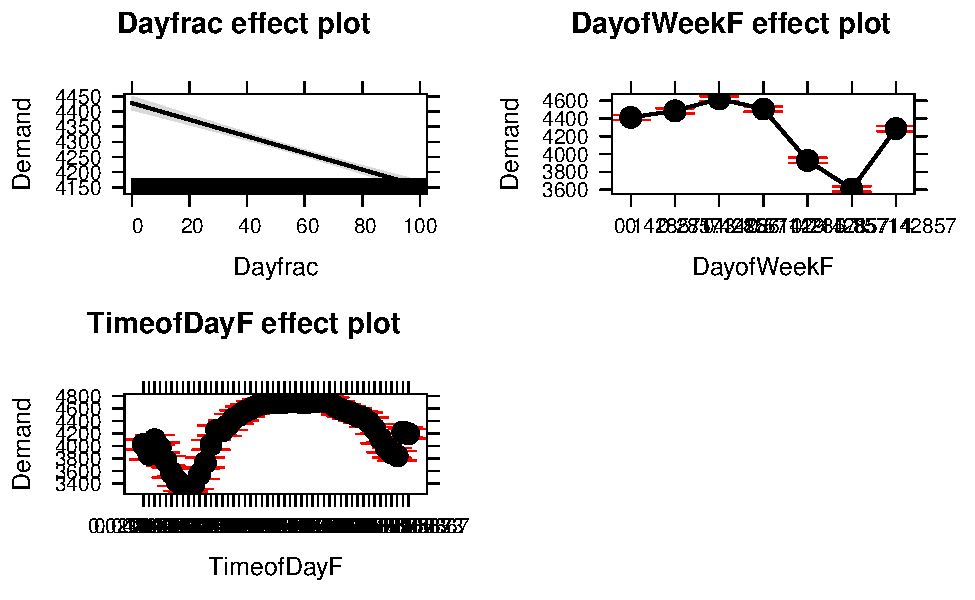
\includegraphics[width=\maxwidth]{figure/prob5c-1} 

}


\begin{kframe}\begin{alltt}
\hlcom{#weekdaystart <- Elec1$time.expanded[1]}

\hlcom{# I need to figure out what time of day the records started.}

\hlstd{tb.daysum} \hlkwb{<-} \hlkwd{table}\hlstd{(Elec1}\hlopt{$}\hlstd{time.expanded, Elec1}\hlopt{$}\hlstd{TimeofDayF)}
\hlstd{mil.hours} \hlkwb{<-} \hlkwd{c}\hlstd{(}\hlstr{"00:30"}\hlstd{,} \hlstr{"1:00"}\hlstd{,} \hlstr{"1:30"}\hlstd{,} \hlstr{"2:00"}\hlstd{,}
               \hlstr{"2:30"}\hlstd{,} \hlstr{"3:00"}\hlstd{,} \hlstr{"3:30"}\hlstd{,} \hlstr{"4:00"}\hlstd{,} \hlstr{"4:30"}\hlstd{,} \hlstr{"5:00"}\hlstd{,} \hlstr{"5:30"}\hlstd{,}
  \hlstr{"6:00"}\hlstd{,} \hlstr{"6:30"}\hlstd{,} \hlstr{"7:00"}\hlstd{,} \hlstr{"7:30"}\hlstd{,} \hlstr{"8:00"}\hlstd{,} \hlstr{"8:30"}\hlstd{,} \hlstr{"9:00"}\hlstd{,}
  \hlstr{"9:30"}\hlstd{,} \hlstr{"10:00"}\hlstd{,} \hlstr{"10:30"}\hlstd{,} \hlstr{"11:00"}\hlstd{,} \hlstr{"11:30"}\hlstd{,}
  \hlstr{"12:00"}\hlstd{,} \hlstr{"12:30"}\hlstd{,}\hlstr{"13:00"}\hlstd{,} \hlstr{"13:30"}\hlstd{,} \hlstr{"14:00"}\hlstd{,} \hlstr{"14:30"}\hlstd{,}
  \hlstr{"15:00"}\hlstd{,} \hlstr{"15:30"}\hlstd{,} \hlstr{"16:00"}\hlstd{,} \hlstr{"16:30"}\hlstd{,} \hlstr{"17:00"}\hlstd{,} \hlstr{"17:30"}\hlstd{,}
  \hlstr{"18:00"}\hlstd{,} \hlstr{"18:30"}\hlstd{,} \hlstr{"19:00"}\hlstd{,} \hlstr{"19:30"}\hlstd{,} \hlstr{"20:00"}\hlstd{,} \hlstr{"20:30"}\hlstd{,}
  \hlstr{"21:00"}\hlstd{,} \hlstr{"21:30"}\hlstd{,} \hlstr{"22:00"}\hlstd{,} \hlstr{"22:30"}\hlstd{,} \hlstr{"23:00"}\hlstd{,} \hlstr{"23:30"}\hlstd{,}
  \hlstr{"24:00"}\hlstd{)}

\hlkwd{colnames}\hlstd{(tb.daysum)} \hlkwb{<-} \hlstd{mil.hours}
\hlkwd{print}\hlstd{(}\hlkwd{xtable}\hlstd{(tb.daysum),} \hlkwc{scalebox} \hlstd{=} \hlnum{0.35}\hlstd{)}
\end{alltt}
\end{kframe}% latex table generated in R 3.3.1 by xtable 1.8-2 package
% Wed Nov 09 15:18:15 2016
\begin{table}[H]
\centering
\scalebox{0.35}{
\begin{tabular}{rrrrrrrrrrrrrrrrrrrrrrrrrrrrrrrrrrrrrrrrrrrrrrrrr}
  \hline
 & 00:30 & 1:00 & 1:30 & 2:00 & 2:30 & 3:00 & 3:30 & 4:00 & 4:30 & 5:00 & 5:30 & 6:00 & 6:30 & 7:00 & 7:30 & 8:00 & 8:30 & 9:00 & 9:30 & 10:00 & 10:30 & 11:00 & 11:30 & 12:00 & 12:30 & 13:00 & 13:30 & 14:00 & 14:30 & 15:00 & 15:30 & 16:00 & 16:30 & 17:00 & 17:30 & 18:00 & 18:30 & 19:00 & 19:30 & 20:00 & 20:30 & 21:00 & 21:30 & 22:00 & 22:30 & 23:00 & 23:30 & 24:00 \\ 
  \hline
Friday &  16 &  16 &  16 &  16 &  17 &  17 &  17 &  16 &  16 &  16 &  16 &  17 &  17 &  17 &  16 &  16 &  16 &  16 &  17 &  17 &  17 &  16 &  16 &  16 &  16 &  17 &  17 &  17 &  16 &  16 &  16 &  16 &  17 &  17 &  17 &  16 &  16 &  16 &  16 &  17 &  17 &  17 &  16 &  16 &  16 &  16 &  17 &  17 \\ 
  Monday &  17 &  17 &  17 &  16 &  16 &  16 &  16 &  17 &  17 &  17 &  16 &  16 &  16 &  16 &  17 &  17 &  17 &  16 &  16 &  16 &  16 &  17 &  17 &  17 &  16 &  16 &  16 &  16 &  17 &  17 &  17 &  16 &  16 &  16 &  16 &  17 &  17 &  17 &  16 &  16 &  16 &  16 &  17 &  17 &  17 &  16 &  16 &  16 \\ 
  Saturda &  17 &  16 &  16 &  16 &  16 &  17 &  17 &  17 &  16 &  16 &  16 &  16 &  17 &  17 &  17 &  16 &  16 &  16 &  16 &  17 &  17 &  17 &  16 &  16 &  16 &  16 &  17 &  17 &  17 &  16 &  16 &  16 &  16 &  17 &  17 &  17 &  16 &  16 &  16 &  16 &  17 &  17 &  17 &  16 &  16 &  16 &  16 &  17 \\ 
  Sunday &  17 &  17 &  16 &  16 &  16 &  16 &  17 &  17 &  17 &  16 &  16 &  16 &  16 &  17 &  17 &  17 &  16 &  16 &  16 &  16 &  17 &  17 &  17 &  16 &  16 &  16 &  16 &  17 &  17 &  17 &  16 &  16 &  16 &  16 &  17 &  17 &  17 &  16 &  16 &  16 &  16 &  17 &  17 &  17 &  16 &  16 &  16 &  16 \\ 
  Thursda &  16 &  16 &  16 &  17 &  17 &  17 &  16 &  16 &  16 &  16 &  17 &  17 &  17 &  16 &  16 &  16 &  16 &  17 &  17 &  17 &  16 &  16 &  16 &  16 &  17 &  17 &  17 &  16 &  16 &  16 &  16 &  17 &  17 &  17 &  16 &  16 &  16 &  16 &  17 &  17 &  17 &  16 &  16 &  16 &  16 &  17 &  17 &  17 \\ 
  Tuesday &  16 &  17 &  17 &  17 &  16 &  16 &  16 &  16 &  17 &  17 &  17 &  16 &  16 &  16 &  16 &  17 &  17 &  17 &  16 &  16 &  16 &  16 &  17 &  17 &  17 &  16 &  16 &  16 &  16 &  17 &  17 &  17 &  16 &  16 &  16 &  16 &  17 &  17 &  17 &  16 &  16 &  16 &  16 &  17 &  17 &  17 &  16 &  16 \\ 
  Wednesd &  16 &  16 &  17 &  17 &  17 &  16 &  16 &  16 &  16 &  17 &  17 &  17 &  16 &  16 &  16 &  16 &  17 &  17 &  17 &  16 &  16 &  16 &  16 &  17 &  17 &  17 &  16 &  16 &  16 &  16 &  17 &  17 &  17 &  16 &  16 &  16 &  16 &  17 &  17 &  17 &  16 &  16 &  16 &  16 &  17 &  17 &  17 &  16 \\ 
   \hline
\end{tabular}
}
\end{table}


Measurements are recorded every 30 minutes of each day of the week. The help file did not state when the 30 minute records began on each day, but for there to be 48 measurements at 30 minute increments for each day, I have to assume that days started at 12 AM each morning. January 10, 2000 was a Monday.

Average demand increased from Monday to Wednesday, hitting its peak on Wednesday. It then decreased until Saturday, with the lowest average (median) demand being on Saturday. Average demand then increased again on Sunday.

Average demand decreased slightly from 12 AM to 12:30 AM, increased again until 1 AM, and then decreased to the seasonal minimum at 4 AM. Average demand then increased until 10:30 AM where the maximum demand was fairly constant from 10:30 AM until 4:30 PM on average. Demand then decreased on average until 10:30 PM where it reached a trough that was slightly lower than the beginning demand. It then increased slightly until 11:30 PM.

\item %5d
{\it Fit a ``gam" model that includes a long-term trend (use thin plate splines and k=10), a day of week cyclic component (use k=7), and a time of day cyclic component (use k=48). Plot each model component and discuss the results for each component including discussing each estimated model component, its p-value, and edf. (6 pts)}

The long term trend had 8.917 edf and has a pvalue of less than 0.001. The trend appears to first decrease, then increase to the peak, followed by a wavey decrease to the trough until right before the end, where it increases again throughout the 115 days displayed.

The day of the week trend had 4.977 edf and is fairly constant, with a slight upward trend until Thursday, where it takes a sharper dive until Saturday, where as it must, it returns to the starting point on Monday. It had a pvalue of less than 0.001.

The time of day spline had 33.985 edf and had a pvalue of less than 0.001. It wiggles and the dives until 5 PM where the spline hits its minimum, it then rises with few wiggles and levels off at the max for much of the day. around 4 PM it decreases more rapidly, wiggles a bit, and reaches the starting point.

The seasonal trends look very similar for the GAM and m1 that was fit.

\begin{knitrout}\footnotesize
\definecolor{shadecolor}{rgb}{1, 1, 1}\color{fgcolor}\begin{kframe}
\begin{alltt}
\hlcom{#make sure all specifications are correct}
\hlstd{gam1} \hlkwb{<-} \hlkwd{gam}\hlstd{(Demand}\hlopt{~}\hlkwd{s}\hlstd{(}\hlkwd{as.vector}\hlstd{(}\hlkwd{time}\hlstd{(Time)),}\hlkwc{k}\hlstd{=}\hlnum{10}\hlstd{,}\hlkwc{bs}\hlstd{=}\hlstr{"ts"}\hlstd{)}\hlopt{+}
              \hlkwd{s}\hlstd{((DayofWeek),}\hlkwc{k}\hlstd{=}\hlnum{7}\hlstd{,}\hlkwc{bs}\hlstd{=}\hlstr{"cc"}\hlstd{)}\hlopt{+}\hlkwd{s}\hlstd{((TimeofDay),}
      \hlkwc{k} \hlstd{=} \hlnum{48}\hlstd{,} \hlkwc{bs} \hlstd{=} \hlstr{"cc"}\hlstd{),} \hlkwc{data}\hlstd{=Elec1,} \hlkwc{family} \hlstd{=} \hlkwd{gaussian}\hlstd{())}

\hlkwd{par}\hlstd{(}\hlkwc{mfrow}\hlstd{=}\hlkwd{c}\hlstd{(}\hlnum{2}\hlstd{,}\hlnum{2}\hlstd{))}
\hlkwd{plot}\hlstd{(gam1)}

\hlkwd{summary}\hlstd{(gam1)}
\end{alltt}
\begin{verbatim}

Family: gaussian 
Link function: identity 

Formula:
Demand ~ s(as.vector(time(Time)), k = 10, bs = "ts") + s((DayofWeek), 
    k = 7, bs = "cc") + s((TimeofDay), k = 48, bs = "cc")

Parametric coefficients:
            Estimate Std. Error t value Pr(>|t|)
(Intercept) 4270.271      5.261   811.6   <2e-16

Approximate significance of smooth terms:
                            edf Ref.df     F p-value
s(as.vector(time(Time)))  8.917      9 167.7  <2e-16
s(DayofWeek)              4.977      5 788.7  <2e-16
s(TimeofDay)             33.985     46 142.2  <2e-16

R-sq.(adj) =  0.686   Deviance explained = 68.9%
GCV = 1.5417e+05  Scale est. = 1.5281e+05  n = 5520
\end{verbatim}
\end{kframe}

{\centering 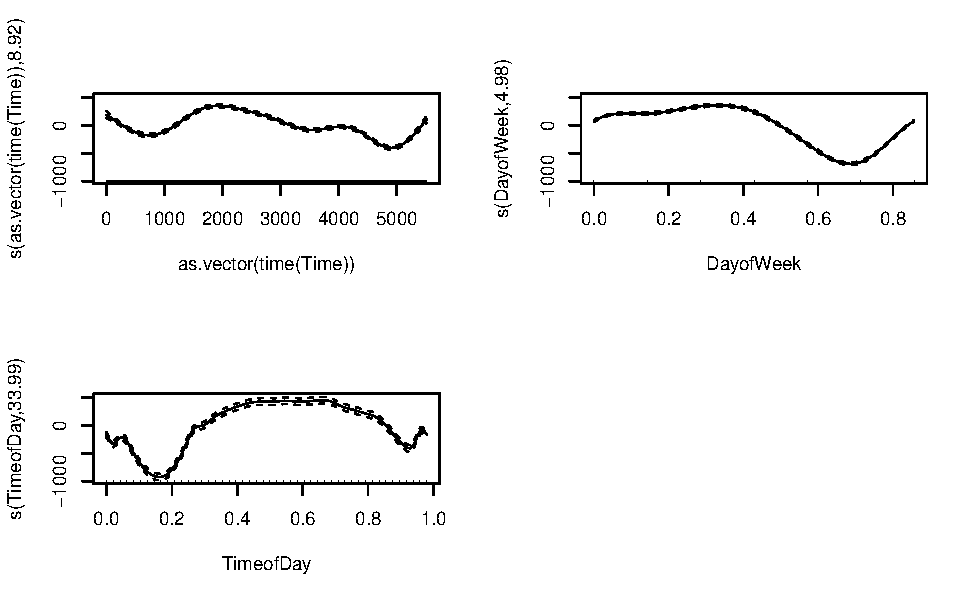
\includegraphics[width=\maxwidth]{figure/prob5d-1} 

}



\end{knitrout}

\item%5e
{\it Compare the AICs for ``m1" and your GAM. Discuss what you learn based on this comparison. (3 pts)
}

The GAM is strongly preferred over the linear long term trend model with seasonality fit as it has an AIC roughly 1000 units smaller and uses a little less than 6 fewer degrees of freedom. It this case, GAM was more efficient and results in a better fit when compared to m1.

\begin{kframe}
\begin{alltt}
\hlstd{aic.elect} \hlkwb{<-} \hlkwd{AIC}\hlstd{(m1,gam1)}

\hlkwd{print}\hlstd{(}\hlkwd{xtable}\hlstd{(aic.elect))}
\end{alltt}
\end{kframe}% latex table generated in R 3.3.1 by xtable 1.8-2 package
% Wed Nov 09 15:18:16 2016
\begin{table}[H]
\centering
\begin{tabular}{rrr}
  \hline
 & df & AIC \\ 
  \hline
m1 & 56.00 & 82670.66 \\ 
  gam1 & 49.88 & 81607.67 \\ 
   \hline
\end{tabular}
\end{table}


\newpage

\item%5f
{\it If there was positive autocorrelation present, would you expect the p-values for your tests for ``m1" to be smaller or larger? Yes or no. No explanation. (1 pt)}

Positive autocorrelation not accounted for will make pvalues smaller than they should be.

\item %5g
{\it With measurements taken every thirty minutes, what is the period of the potential weekly seasonal component in terms of number of observations? The potential daily seasonal component? Make sure you report the units of the response (blank per blank). (3 pts) }

With observations taken every 30 minutes and a weekly period, there are 48*7 = 336 observations per weekly period.

Each potential daily seasonal component has 48 observations per day.


\end{enumerate}
\end{enumerate}

\end{document}
